\documentclass{beamer}
\usepackage{xcolor}
\usepackage{natbib} % package to organize literature
\usepackage{multicol}
\usepackage{booktabs}
\usepackage{wasysym} % additional symbols
\usepackage{graphicx} % to include graphics, gifs
\usepackage{color} % add colored text
\usepackage{lmodern} % to fix font size error, might be problematic with math symbols
\usepackage{array}

\usetheme{Frankfurt}
\usecolortheme{beaver}
\setbeamertemplate{footline}
{
  \leavevmode%
  \hbox{%
  \begin{beamercolorbox}[wd=.3\paperwidth,ht=2.25ex,dp=1ex,center]{author in head/foot}%
    \usebeamerfont{author in head/foot}\insertshortauthor \hspace{1em} (\insertshortinstitute)
  \end{beamercolorbox}%
  \begin{beamercolorbox}[wd=.4\paperwidth,ht=2.25ex,dp=1ex,center]{title in head/foot}%
    \usebeamerfont{title in head/foot}\insertshorttitle
  \end{beamercolorbox}%
  \begin{beamercolorbox}[wd=.3\paperwidth,ht=2.25ex,dp=1ex,right]{author in head/foot}%
    \usebeamerfont{author in head/foot}\insertdate \hspace{2em}
    \insertframenumber{} / \inserttotalframenumber\hspace*{1em}
  \end{beamercolorbox}}%
  \vskip0pt%
}
%\definecolor{beamer@sbred}{rgb}{0.65,0.15,0.18}
\definecolor{beamer@sbred}{rgb}{0.22,0.22,0.66}
\setbeamercolor{title}{fg=beamer@sbred,bg=black!5}
\setbeamercolor{structure}{fg=beamer@sbred}
\setbeamercolor{frametitle}{fg=beamer@sbred}
\setbeamercolor{palette primary}{fg=beamer@sbred,bg=black!10}
\setbeamercolor{palette secondary}{fg=beamer@sbred}
\setbeamercolor{palette tertiary}{bg=beamer@sbred}
\setbeamercolor{palette quaternary}{fg=white,bg=beamer@sbred}
\setbeamertemplate{itemize items}[default]
\setbeamertemplate{enumerate items}[default]
\setbeamersize{text margin left=1em,text margin right=1em}
\DeclareTextFontCommand{\emph}{\color{beamer@sbred}}

\author[Patrick Kraft]{Patrick Kraft}
\institute[Stony Brook]{Graduate Student Colloquium}
\title[Voter Utilities and Majority Voting]{Moral Foundations of Political Reasoning \\ {\small Investigating the Moral Underpinnings of Political Judgment}}
\date{October 21, 2014}
\titlegraphic{\includegraphics[width=4cm]{/data/Dropbox/1-src/logos/logo_bk.pdf}}

\begin{document}
\frame{\titlepage}
%\footnotesize


\section{Introduction}
\subsection{}
\begin{frame}%[allowframbreaks]
  \frametitle{Questions}
  \begin{itemize}
    \item Do individuals rely on \emph{moral foundations} when evaluating political \emph{parties} and \emph{candidates}?
    \item Are there systematic differences between \emph{liberals} and \emph{conservatives}?
    \item Are moral values \emph{determinants} of political thinking, or only a \emph{rhetorical device} that citizens learn to bolster their political views?
  \end{itemize}
\end{frame}

\section{}
\subsection{}
\begin{frame}%[allowframbreaks]
  \frametitle{Moral Foundations Theory}
  \begin{itemize}
    \item Moral thinking is structured by 5 central \emph{innate intuitions} \citep{haidt2008moral}:
    \begin{itemize}
      \item Harm / Care
      \item Fairness / Reciprocity
      \item Ingroup / Loyalty
      \item Authority / Respect
      \item Purity / Sanctity
    \end{itemize}
    \item \emph{Liberals} and \emph{conservatives} rely on different sets of moral foundations \citep[e.g][]{graham2009liberals,haidt2007morality}
  \end{itemize}
\end{frame}

\section{}
\subsection{}
\begin{frame}%[allowframbreaks]
  \frametitle{Hypotheses}
  \begin{enumerate}
    \item \emph{Liberals} are more likely to emphasize moral foundations of \emph{harm/care} and \emph{fairness/reciprocity} than conservatives when evaluating political parties and candidates. On the other hand, \emph{conservatives} are more likely to emphasize moral foundations of \emph{ingroup/loyalty}, \emph{authority/respect}, and \emph{purity/sanctity} than liberals.
    \item The ideological differences in references to moral foundations are \emph{moderated by individual political interest}. Higher political interest increases the gap between liberals and conservatives in their relative emphasis on the moral foundations described in hypothesis 1.
  \end{enumerate}
\end{frame}

\section{Empirical Analyses}
\subsection{}
\begin{frame}%[allowframbreaks]
  \frametitle{Overview}
  \begin{itemize}
    \item 2012 American National Election Study (pre-election)
    \item Computer assisted face-to-face interviews + Internet panel
    \item Major dependent variable: \emph{open-ended questions} where respondents were asked what they \emph{liked} and \emph{disliked} about the parties and candidates
    \item Moral Foundations \emph{dictionary} proposed by \citep{graham2009liberals} to look for \emph{signal} words.
    \item Model individual response patterns for each of the moral foundations
  \end{itemize}
\end{frame}

\subsection{}
\begin{frame}%[allowframbreaks]
  \frametitle{Analyzing Open-Ended Survey Responses}
  \begin{itemize}
    \item \emph{Example}: \textit{Is there anything in particular about Barack Obama that might make you want to vote for him? What is that?}
    \item \emph{\textit{Original statement}}:
    \begin{center}
      ``He has \underline{qulification} to be a leader, things he has accomplished he is qualified to be a leader, for women rights doing something for middle class''
    \end{center}
    \item \emph{\textit{Processed statement}}:
    \begin{center}
      ``he has \underline{qualification} to be a {\color{red}leader} things he has accomplished he is qualified to be a {\color{red}leader} for women {\color{green}rights} doing something for middle {\color{red}class}''
    \end{center}
  \item \emph{\textit{Moral Foundations}}: {\color{red}Authority}, {\color{green}Fairness}
  \end{itemize}
\end{frame}

\subsection{}
\begin{frame}%[allowframbreaks]
  \frametitle{Descriptive Results I}
  \begin{figure}[ht]\centering
    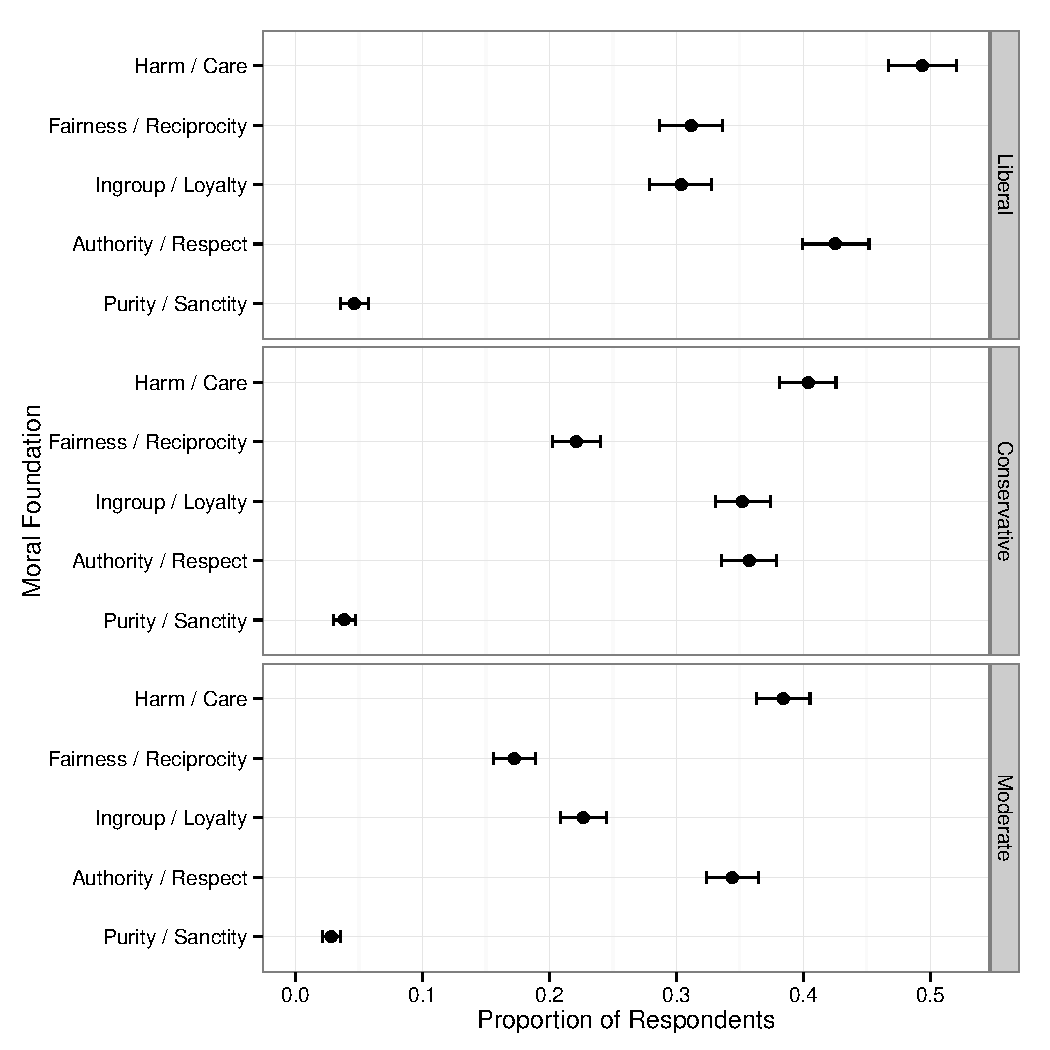
\includegraphics[height=.75\textheight]{p1_mft_ideol}
    \caption{Moral Foundations and Ideology (All Statements)}
  \end{figure}
\end{frame}

\begin{frame}%[allowframbreaks]
  \frametitle{Descriptive Results II}
  \begin{figure}[ht]\centering
    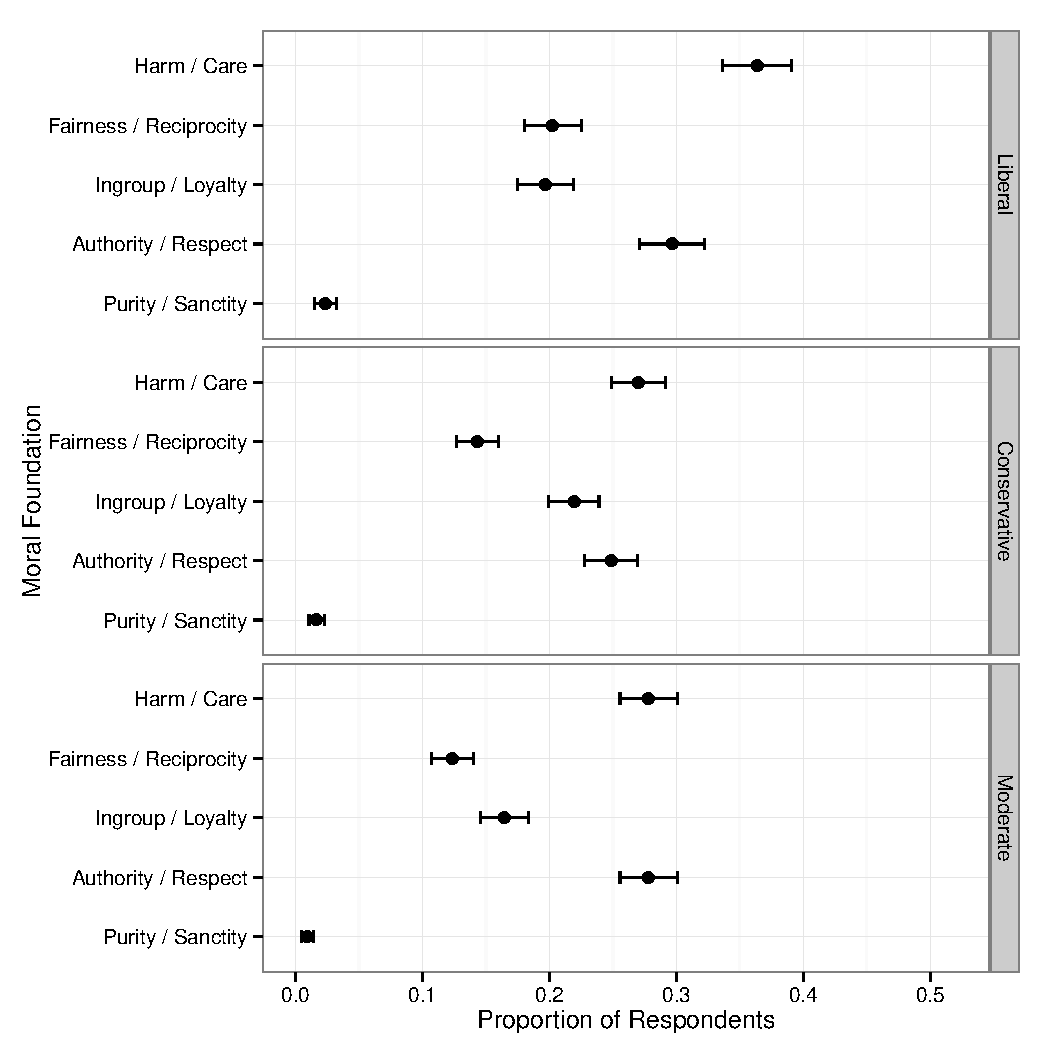
\includegraphics[height=.75\textheight]{p2_mft_ideol_pa}
    \caption{Moral Foundations and Ideology (Party Evaluations)}
  \end{figure}
\end{frame}

\begin{frame}%[allowframbreaks]
  \frametitle{Descriptive Results III}
  \begin{figure}[ht]\centering
    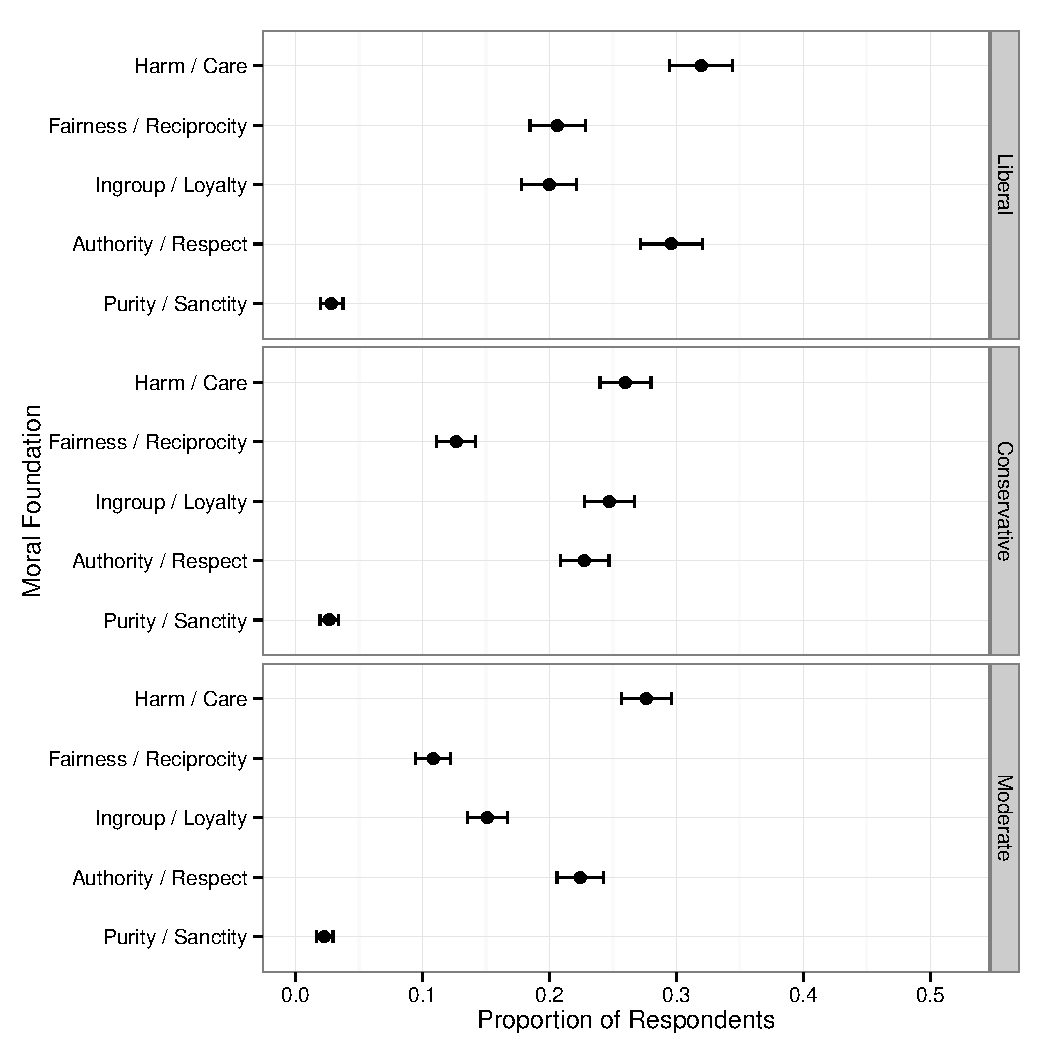
\includegraphics[height=.75\textheight]{p3_mft_ideol_ca}
    \caption{Moral Foundations and Ideology (Candidate Evaluations)}
  \end{figure}
\end{frame}

\subsection{}
\begin{frame}%[allowframbreaks]
  \frametitle{Logit Model I - Model Specification}
  \begin{align*}
    P(\text{MF}) = \text{logit}^{-1}(&\beta_0+\beta_1C+\beta_2M + \beta_3PI \\
    &+ \beta_5 C*PI + \beta_6 M*PI \\
    &+ \beta\mathbf{X})
  \end{align*}
  \begin{itemize}
    \item \emph{Controls}: Church attendance, education, age, gender, race
  \end{itemize}
\end{frame}

\begin{frame}%[allowframbreaks]
  \frametitle{Logit Model II - Results}
  \begin{figure}[ht]\centering
    \includegraphics[height=.75\textheight]{p4_models}
    \caption{Moral Foundations and Ideology (Candidate Evaluations)}
  \end{figure}
\end{frame}

\subsection{}
\begin{frame}%[allowframbreaks]
  \frametitle{Potential Improvements and Future Analyses}
  \begin{itemize}
    \item Control for answer length (!)
    \item Other ways to demonstrate that moral foundations are universal. Experimental designs?
    \item Revise dictionary
    \item Multi-dimensional conceptualization of ideology?
    \item Measure of political sophistication?
    \item Differentiate between rejection and approval to moral foundations?
    \item Differentiate between in-party / out-party, candidate vs. party, etc.
    \item Effects of campaign exposure, political discussion etc.
    \item Structural topic models \citep{roberts2014structural}

  \end{itemize}
\end{frame}

\section{Appendix}
\subsection{}
\begin{frame}%[allowframbreaks]
  \frametitle{Moral Foundations Dictionary \citep[c.f.][]{graham2009liberals}}
  \begin{tiny}
    \begin{itemize}
      \item \emph{Harm:} safe*, peace*, compassion*, empath*, sympath*, care, caring, protect*, shield, shelter, amity, secur*, benefit*, defen*, guard*, preserve, harm*, suffer*, war, wars, warl*, warring, fight*, violen*, hurt*, kill, kills, killer*, killed, killing, endanger*, cruel*, brutal*, abuse*, damag*, ruin*, ravage, detriment*, crush*, attack*, annihilate*, destroy, stomp, abandon*, spurn, impair, exploit, exploits, exploited, exploiting, wound*

      \item \emph{Fairness:} fair, fairly, fairness, fair*, fairmind*, fairplay, equal*, justice, justness, justifi*, reciproc*, impartial*, egalitar*, rights, equity, evenness, equivalent, unbias*, tolerant, equable, balance*, homologous, unprejudice*, reasonable, constant, honest*, unfair*, unequal*, bias*, unjust*, injust*, bigot*, discriminat*, disproportion*, inequitable, prejud*, dishonest, unscrupulous, dissociate, preference, favoritism, segregat*, exclusion, exclud*

      \item \emph{Ingroup:} together, nation*, homeland*, family, families, familial, group, loyal*, patriot*, communal, commune*, communit*, communis*, comrad*, cadre, collectiv*, joint, unison, unite*, fellow*, guild, solidarity, devot*, member, cliqu*, cohort, ally, insider, foreign*, enem*, betray*, treason*, traitor*, treacher*, disloyal*, individual*, apostasy, apostate, deserted, deserter*, deserting, deceiv*, jilt*, imposter, miscreant, spy, sequester, renegade, terroris*, immigra*

      \item \emph{Authority:} obey*, obedien*, duty, law, lawful*, legal*, duti*, honor*, respect, respectful*, respected, respects, order*, father*, mother, motherl*, mothering, mothers, tradition*, hierarch*, authorit*, permit, permission, status*, rank*, leader*, class, bourgeoisie, caste*, position, complian*, command, supremacy, control, submi*, allegian*, serve, abide, defere*, defer, revere*, venerat*, comply, defian*, rebel*, dissent*, subver*, disrespect*, disobe*, sediti*, agitat*, insubordinat*, illegal*, lawless*, insurgent, mutinous, defy*, dissident, unfaithful, alienate, defector, heretic*, nonconformist, oppose, protest, refuse, denounce, remonstrate, riot*, obstruct

      \item \emph{Purity:} piety, pious, purity, pure*, clean*, steril*, sacred*, chast*, holy, holiness, saint*, wholesome*, celiba*, abstention, virgin, virgins, virginity, virginal, austerity, integrity, modesty, abstinen*, abstemiousness, upright, limpid, unadulterated, maiden, virtuous, refined, intemperate, decen*, immaculate, innocent, pristine, humble, disgust*, deprav*, disease*, unclean*, contagio*, indecen*, sin, sinful*, sinner*, sins, sinned, sinning, slut*, whore, dirt*, impiety, impious, profan*, gross, repuls*, sick*, promiscu*, lewd*, adulter*, debauche*, defile*, tramp, prostitut*, unchaste, wanton, profligate, filth*, trashy, obscen*, lax, taint*, stain*, tarnish*, debase*, desecrat*, wicked*, blemish, exploitat*, pervert, wretched*
    \end{itemize}
  \end{tiny}
\end{frame}

\subsection{}
\begin{frame}
  \frametitle{References}
  \def\newblock{\hskip .11em plus .33em minus .07em}
  %\nocite{*}
  \begin{scriptsize}
    \bibliographystyle{apsr}
    \bibliography{/data/Dropbox/1-src/lit/Literature}
  \end{scriptsize}
\end{frame}

\end{document}